\chapter{Protótipos}
\label{chap:proto}
%A description of all (functional and non-functional) prototypes developed together with an explanation of their development path (e.g., a discussion of any alternatives that were considered).

É de notar que a concepção do projecto começou com ideias baseadas na \textit{Cloud} e nos perigos subjacentes ao seu uso,
ideias essas que, no decorrer no projecto, foram mudando e tomando outras formas,
como pode ser visto pelo facto de que o objectivo do projecto descrito na Introdução (Capítulo \ref{chap:intro}) já não mencionar a \textit{Cloud}.
Apesar disso muitos protótipos desenvolvidos ainda tinham como base a ideia original.

\section{Prótotipos Não-Funcionais}
A construção dos protótipos começou após uma reunião de grupo, onde se acordou que cada elemento criaria 2 (dois) protótipos não-funcionais para um jogo que eles achassem que passasse bem a mensagem, estes foram os resultados.
\subsection{Protótipos do Ricardo}

\begin{figure}[h]
\centering
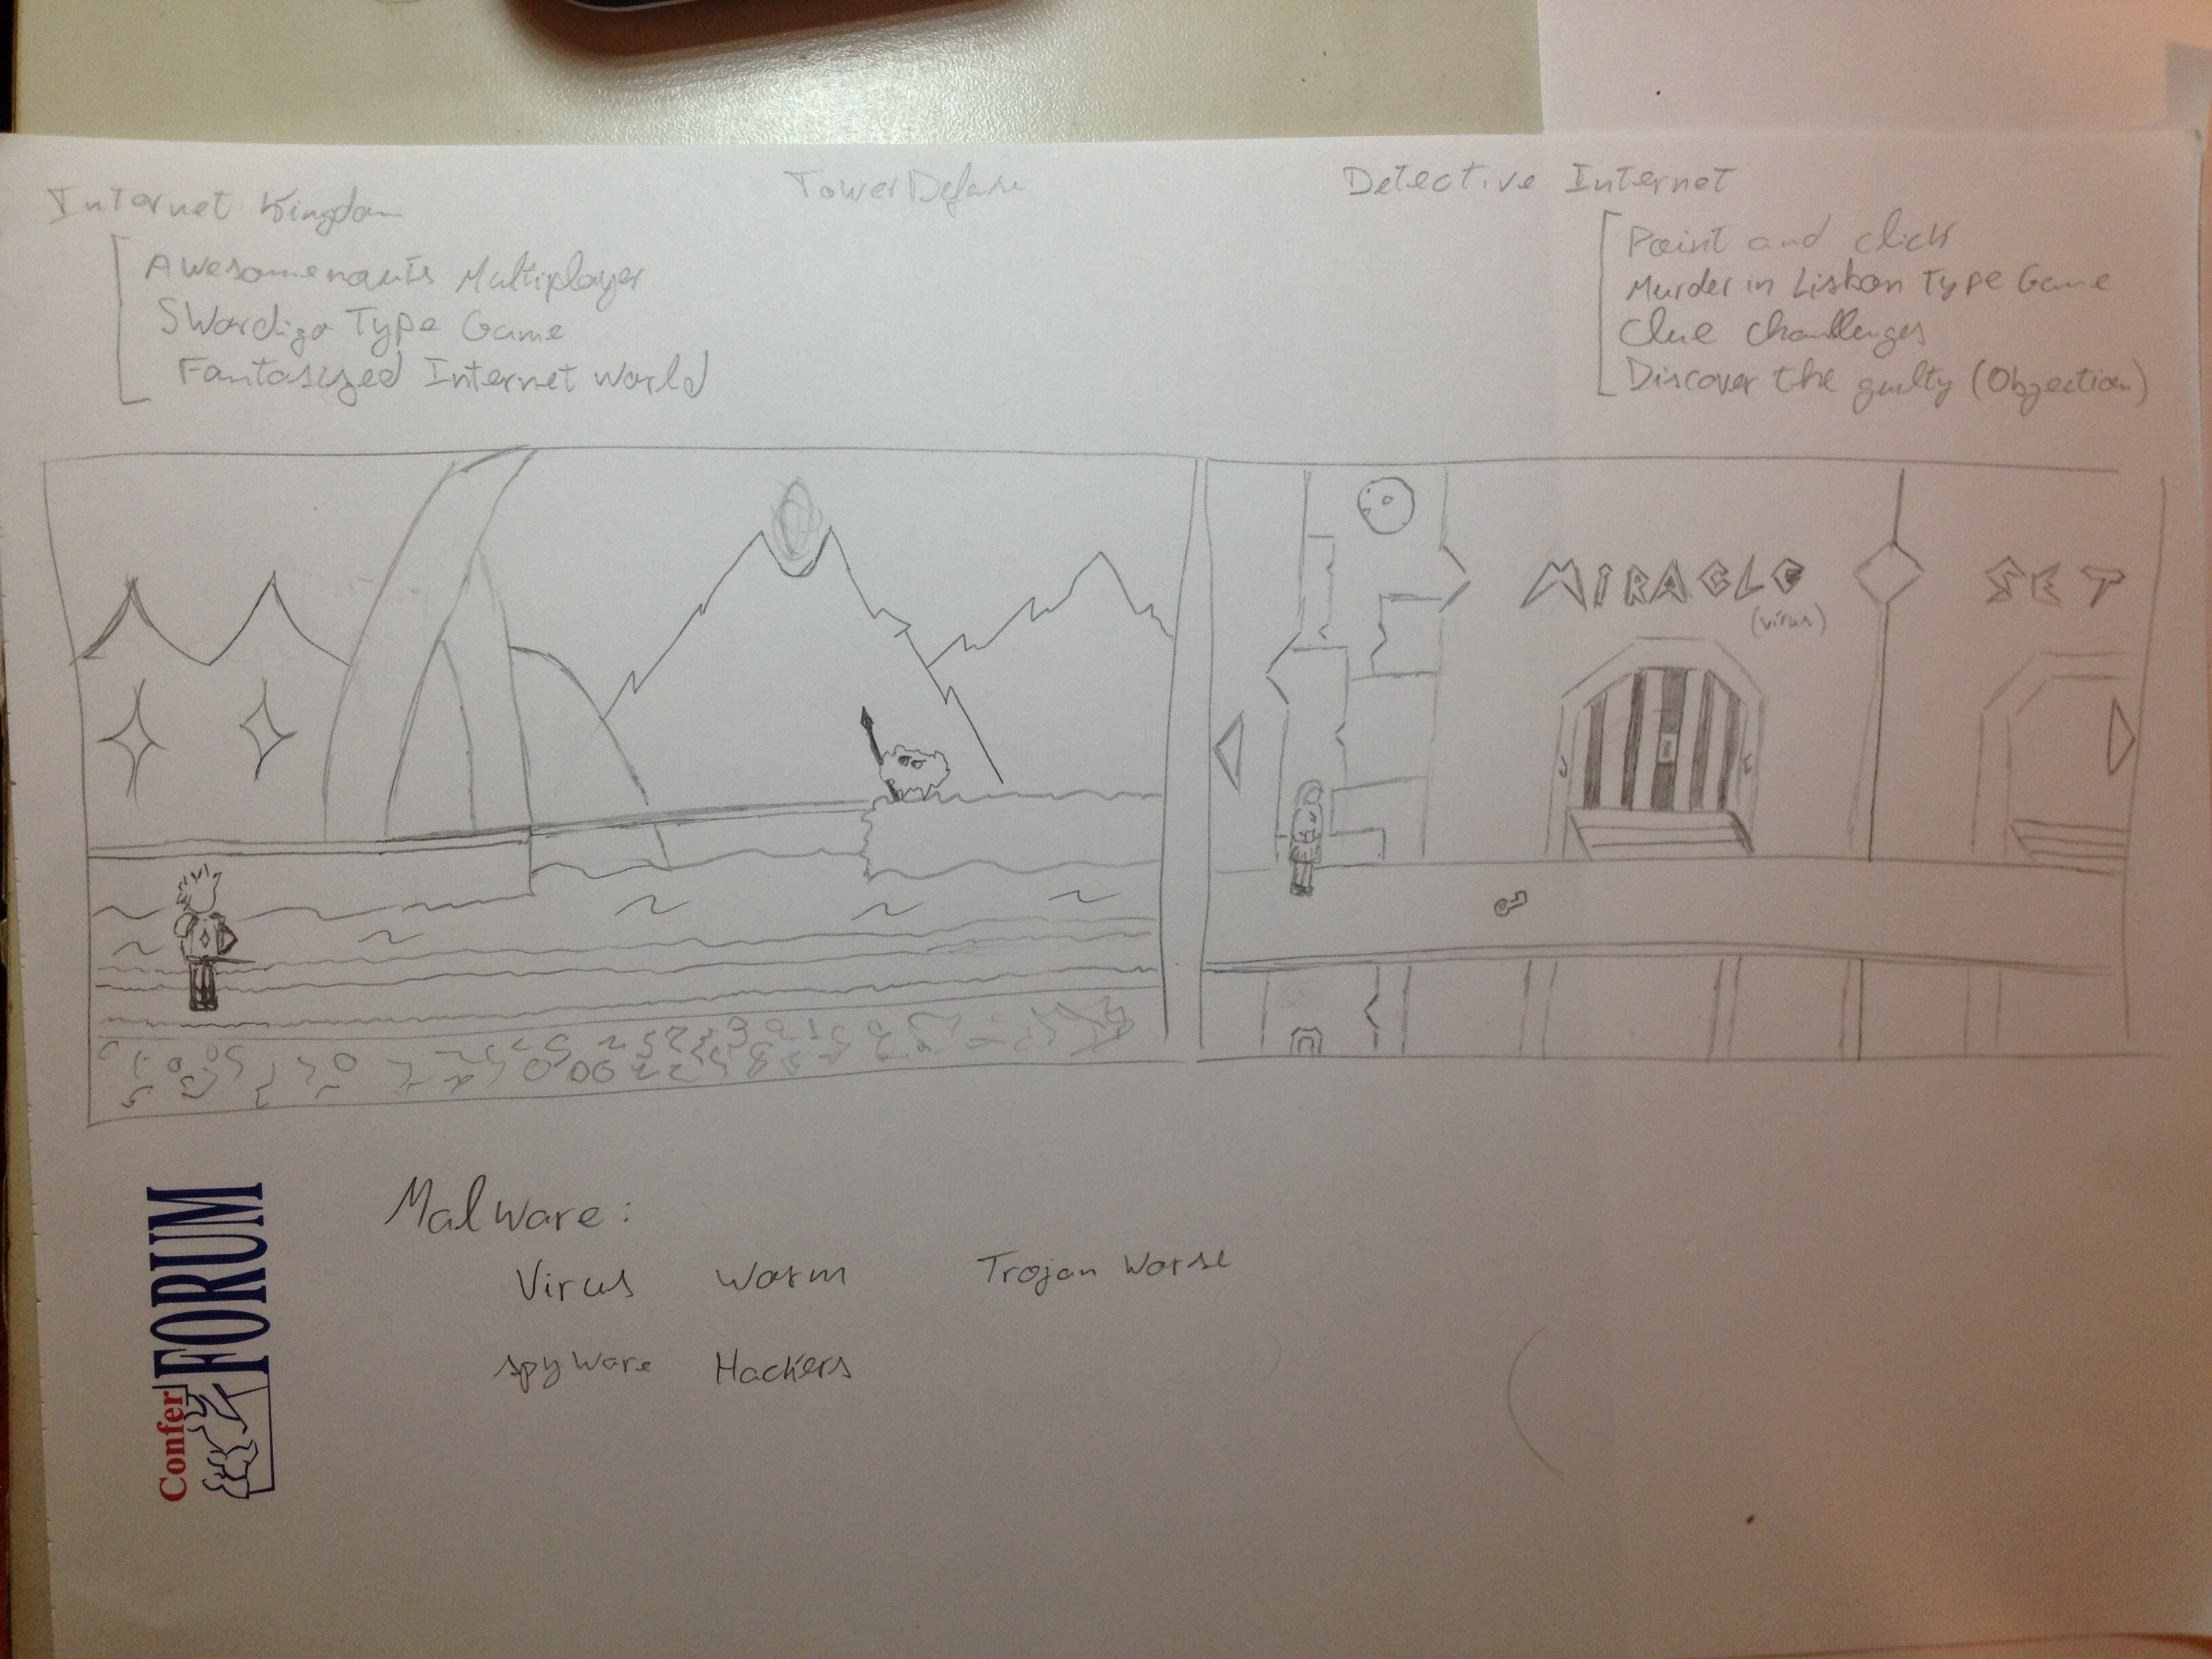
\includegraphics 
	[width = 0.75\textwidth] {Ricardo/ricardo_prototipo_1}
\caption{\label{fig:ric:prot1}} Protótipos do Ricardo
\end{figure}

Estes protótipos visavam jogos bastante diferentes. No lado esquerdo da Figura \ref{fig:ric:prot1} vemos um jogo ao estilo \textit{Hack and Slash}, o ideia por detrás deste jogo é que o jogador seria uma \textit{Ciber-Guardião} que defenderia a sua rede local de ataques de \textit{Malwares}, e a cada passo da história ir-se-ia descobrindo novos \textit{Malwares} e como nos proteger-mos deles.

Por sua vez, no lado direito da Figura \ref{fig:ric:prot1}, vemos um jogo de investigação, em que uma nova navegante da Internet teria de embarcar numa aventura para descobrir a entidade de um famoso \textit{Hacker}, que estava a destruir servidores e a espalhar medo pela Internet fora, e parar o seu reino de terror.
Ao longo do jogo, o jogador ia descobrindo os perigos dos \textit{Malwares} e como se proteger.

\subsection{Protótipos do Tiago}



\subsection{Protótipos do Ian}

O primeiro protótipo (Figura \ref{fig:ian:prot1}) foi um rail-shooter, onde se controlava uma nave, que transportava uma mensagem importante, e disparava caracteres de password. O objectivo seria levar a mensagem de um ponto a outro, protegendo-a de vários \textit{Vírus} e \textit{bosses} que iriam aparecendo ao longo dos níveis. Seria também possível apanhar \textit{power ups}, como escudos de Antivírus. Haveria dois modos, um modo campanha que seria uma série de níveis, e um modo infinito, que seria um nível que apenas acabaria quando o jogador ficasse sem vidas. Este modo infinito permitiria guardar a pontuação numa tabela para comparar com a de outros jogadores.

\begin{figure}[h]
\centering
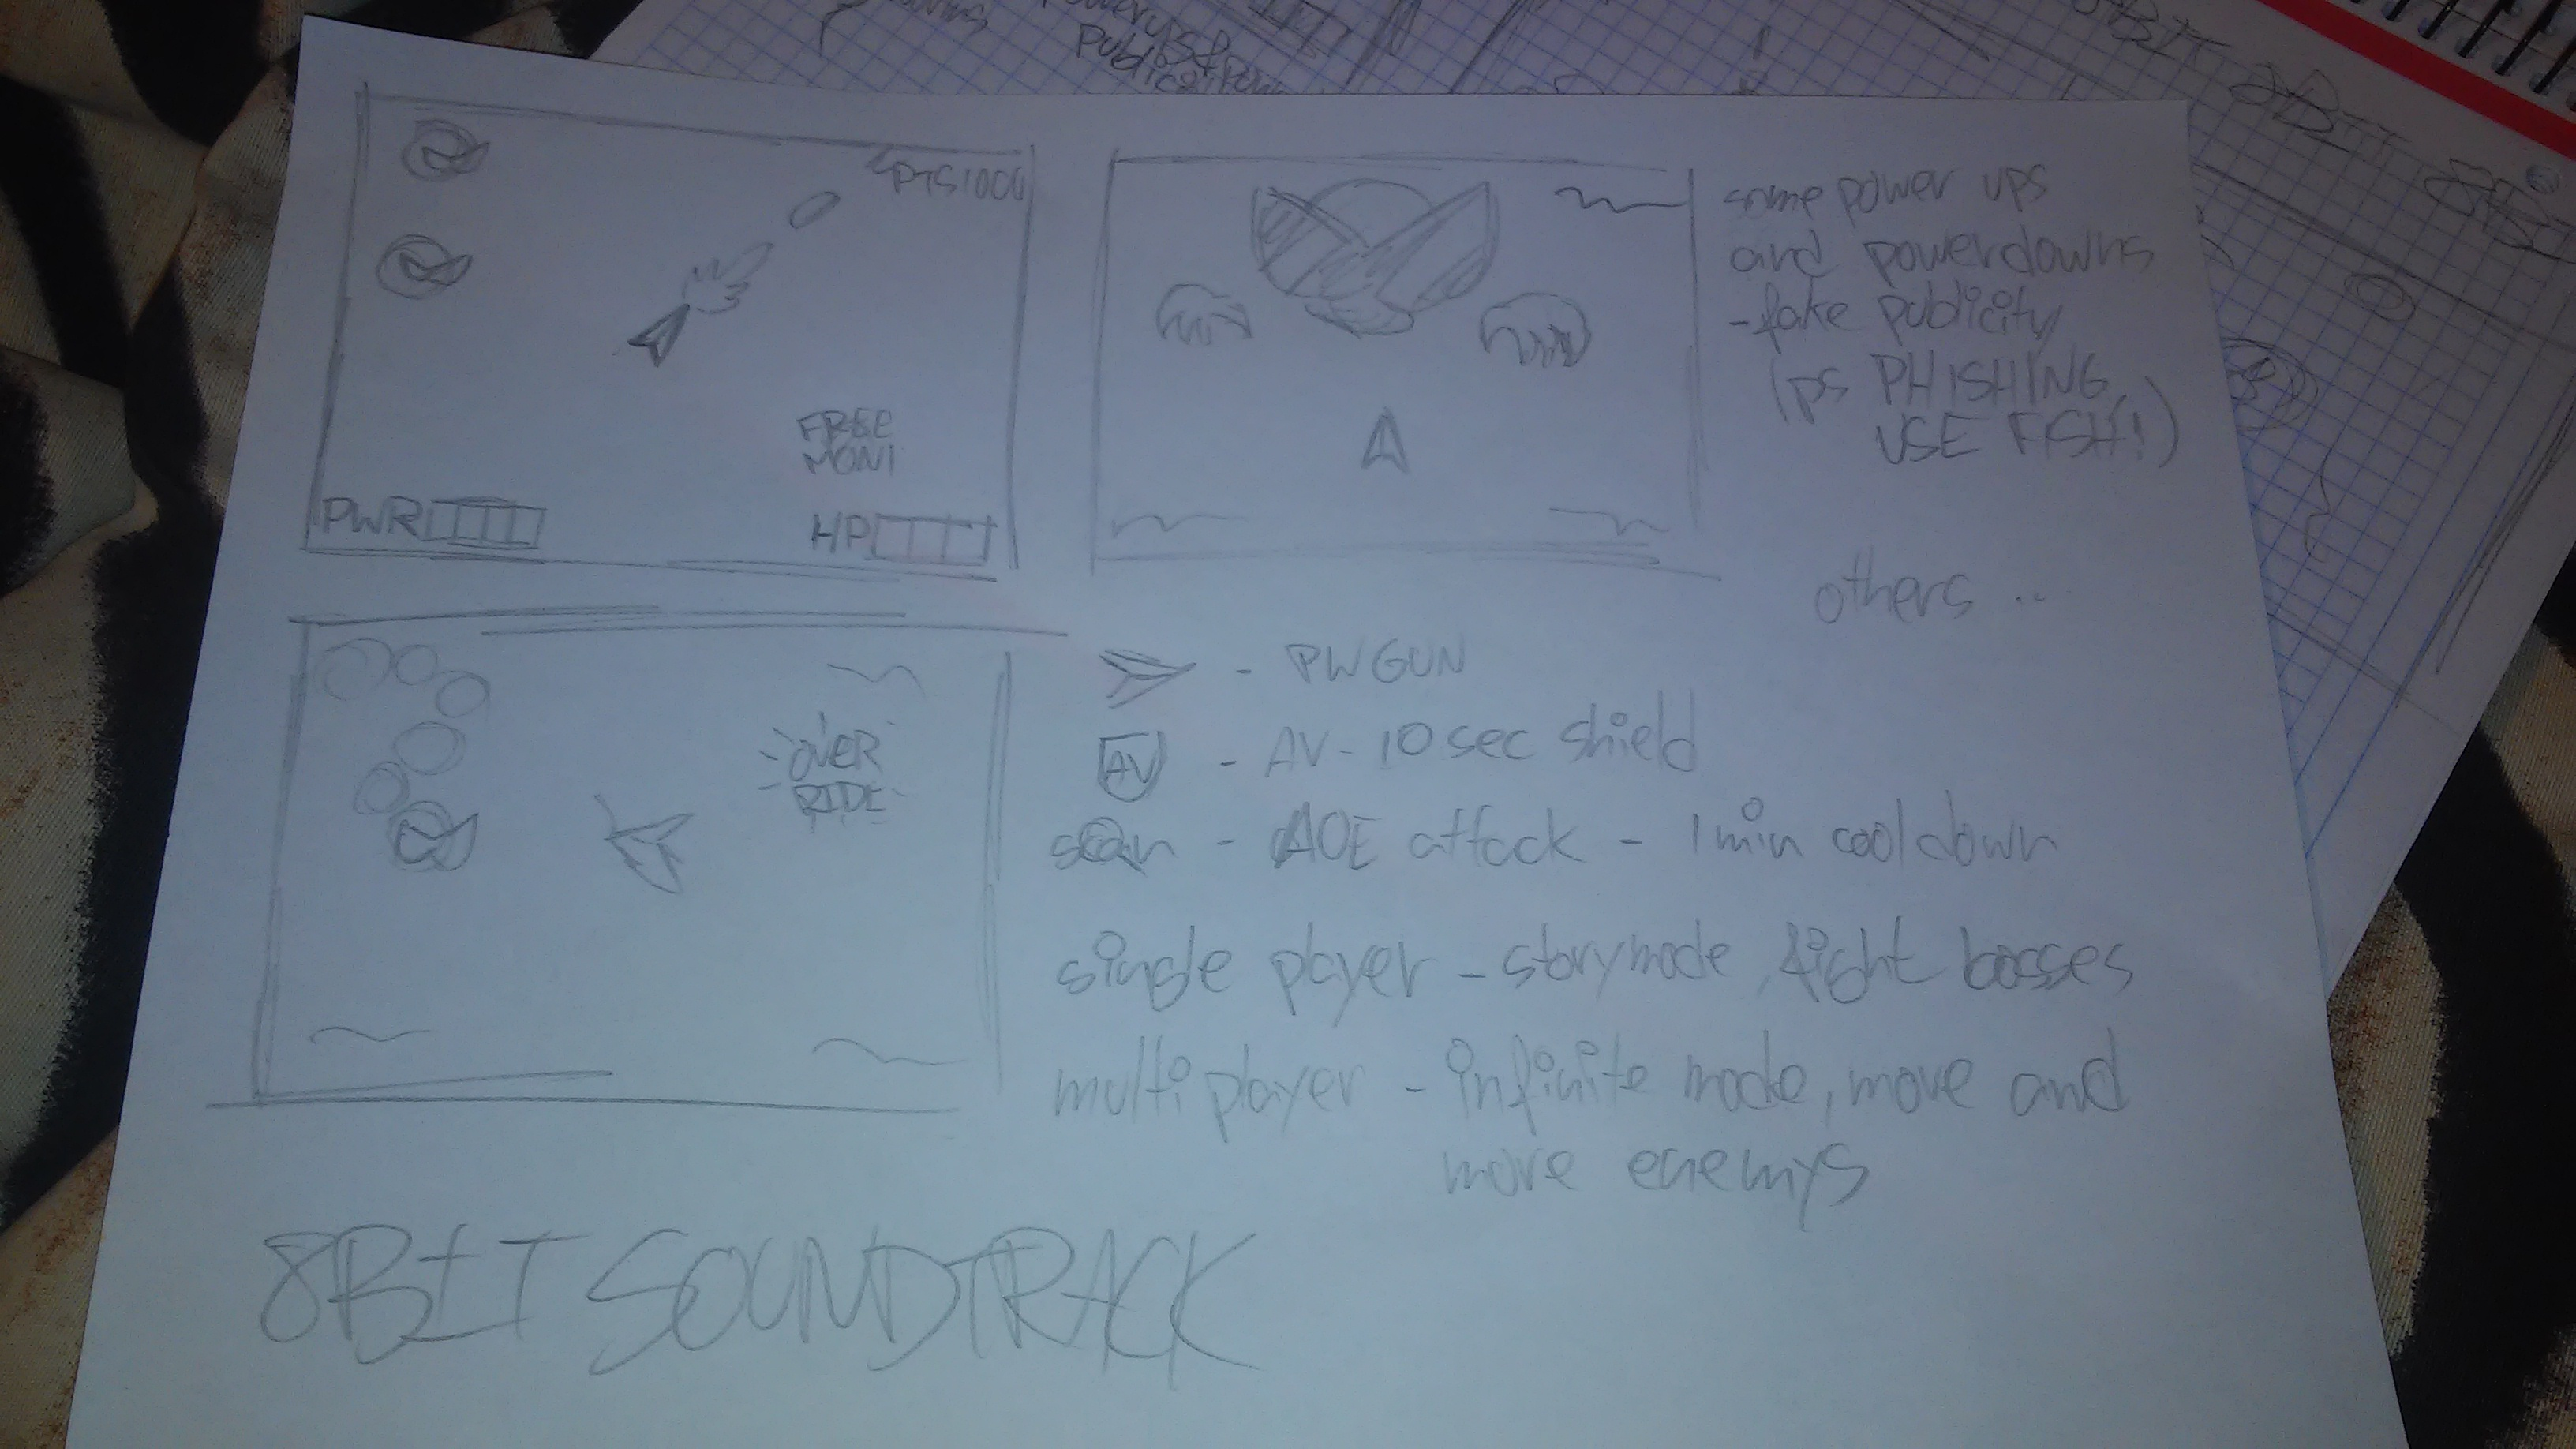
\includegraphics 
	[width = 0.75\textwidth] {Ian/ian_prototipo_1}
\caption{\label{fig:ian:prot1}} Primeiro Protótipo do Ian
\end{figure}

O segundo protótipo (Figura \ref{fig:ian:prot2}) era um \textit{God Game}, onde o jogador controlava um Deus das Nuvens (\textit{Clouds}). Esse Deus seria venerado inicialmente por uma vila, e o objectivo seria expandir essa vila, ganhando assim pontos. Com estes pontos seria possível desbloquear poderes, como por exemplo \textit{Firewalls} para proteger a vila de inimigos. Os inimigos poderiam ser vários tipo de vírus (\textit{Worms} seriam representados por serpentes gigantes, \textit{Trojans} cavalos, etc), ou outras vilas hostis, representando \textit{Hackers}. A movimentação dos habitantes pelas vilas seriam assim uma metáfora para a troca do informação pela \textit{Cloud}, e a expansão da vila o crescimento da \textit{Cloud}.

\begin{figure}[h]
\centering
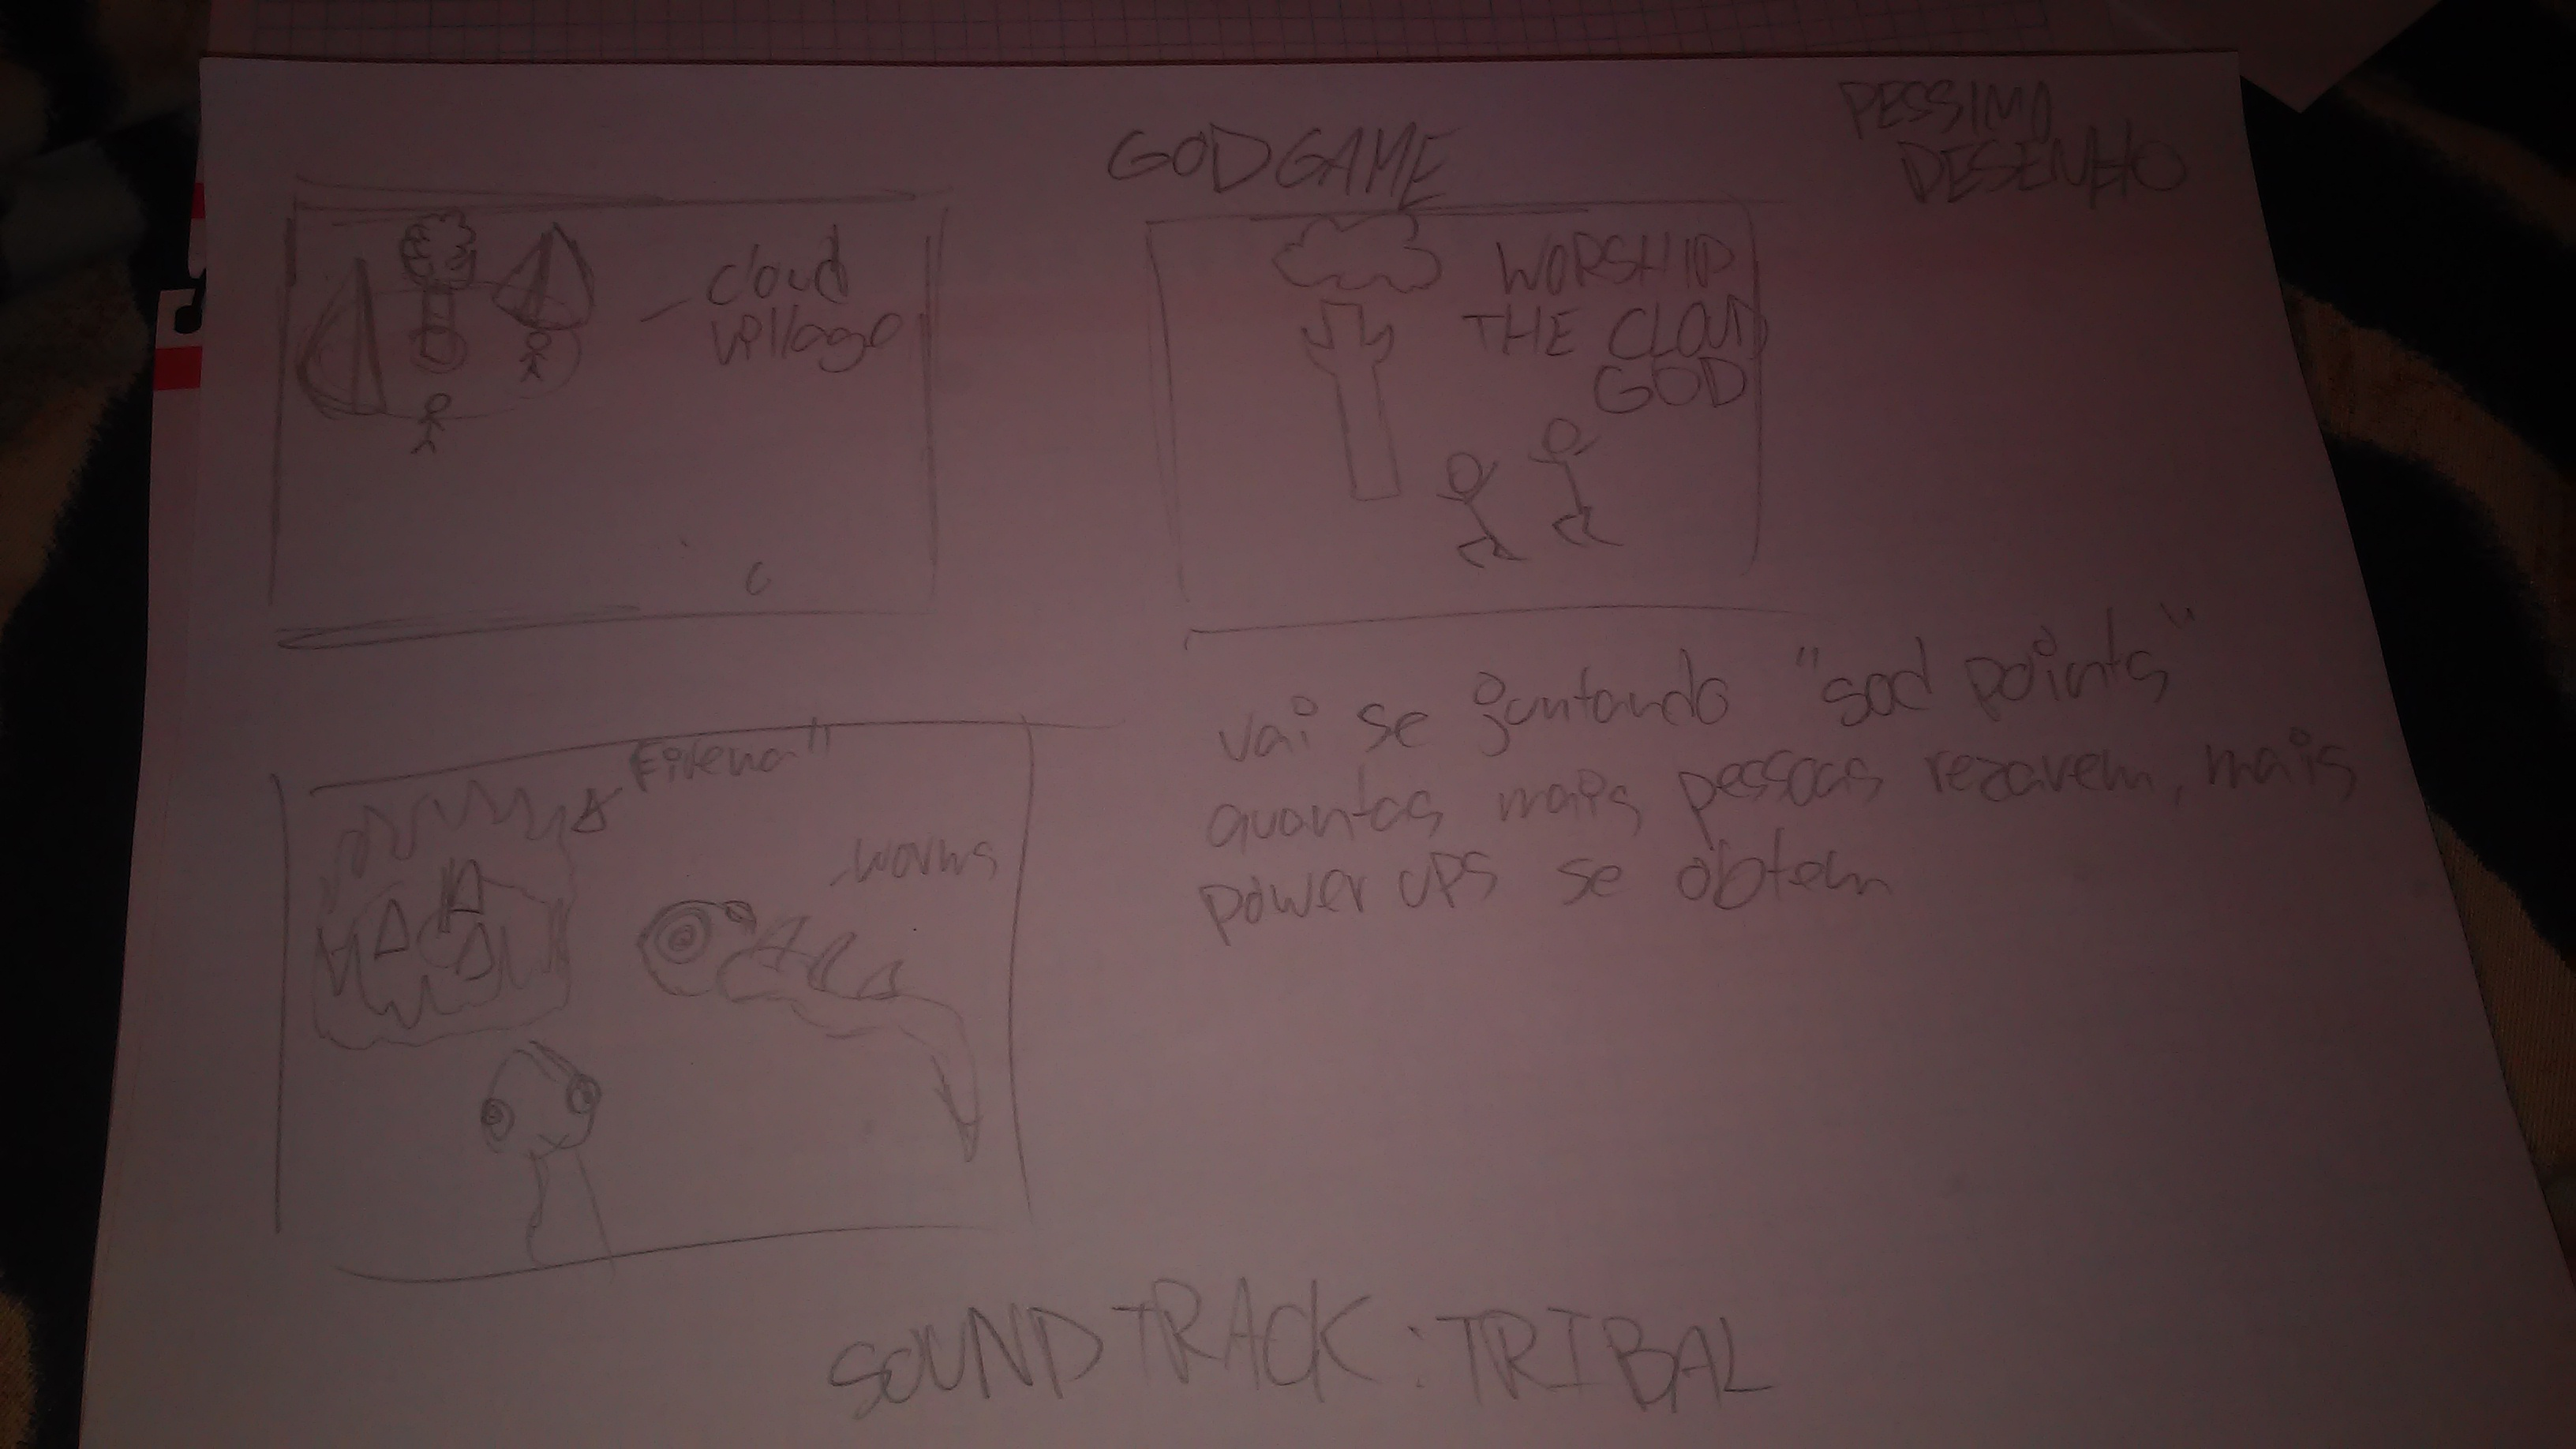
\includegraphics 
	[width = \textwidth] {Ian/ian_prototipo_2}
\caption{\label{fig:ian:prot2}} Segundo Protótipo do Ian
\end{figure}

\subsection{A Escolha}

Depois de cada elemento ter revelado os seus protótipos, foi feita uma escolha de qual deles seria usado para futuros passos, como a criação de um protótipo funcional.

Os protótipos que mais chamaram à atenção, pela sua criatividade e possíveis dinâmicas de jogo, foram o \textit{God Game}, que oferecia uma metáfora forte sobre a \textit{Cloud} e \textit{Malwares}, e o \textit{Hack and Slash}, que mostrava um jogo maior e mais complexo que implicava uma evolução da personagem e uma história forte. Infelizmente, por falta de conhecimentos para criar projectos assim tão grandes, decidiu-se optar por soluções mais pequenas.

Assim, as possíveis escolhas foram o \textit{Railshooter} e o \textit{Platformer}, quer

\section{Protótipos de Baixa Fidelidade}

Depois dos protótipos não-funcionais serem apresentados 